% !TEX root = ../main.tex
\begin{figure}[t]
  \centering
  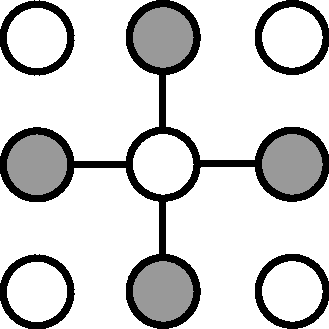
\includegraphics[height=0.2\paperheight]{fig/ising-markov-blanket.pdf}
  \caption[Markov blanket of a node in an Ising model]{
  \textbf{The structure of an Ising model can inform variational approximations.} This graphical model illustrates a Markov blanket in the Ising model of \Cref{fig:graphical-model-ising}. The Markov blanket of a node is the set of nodes whose values need to be fixed to render a node independent of the rest of the graph. In an Ising model, only neighboring random variables interact and therefore comprise the Markov blanket of a node. Here, the Markov blanket of the central node are shaded, indicating that their values are fixed. The missing edges between the peripheral nodes indicate that the central node is independent of the rest of the graph, conditional on its Markov blanket.}
  \label{fig:ising-markov-blanket}
\end{figure}